\documentclass[english]{tktltiki}
\usepackage[pdftex]{graphicx}
\usepackage{subfigure}
\usepackage{url}
\begin{document}
%\doublespacing
%\singlespacing
\onehalfspacing

\title{Assignment 3: Interaction prototyping for a handheld device}
\author{P�ter Ivanics}
\date{\today}

\maketitle

\numberofpagesinformation{\numberofpages\ pages + \numberofappendixpages\ appendices}
\keywords{}

\mytableofcontents

\section{Introduction}
	This report is a summary of the process on prototyping a restaurant-finder mobile application. The report is rolled out as one of the assignment of the Human-Computer Interaction course and serves the purpose to gain hands-on experience with the course material. 
	
	The goal of this report and assignment is to gain hands-on experience with paper-based prototyping and storyboarding of a mobile application. As a case study, the design of a simple restaurant finder mobile application is given and is described in this report. The initial prototypes, proposals and storyboards are displayed and briefly described in the following chapter. Further, some conclusions are derived and future improvements are suggested. 
	
\section{Discussion}
	\subsection{Sketches and Storyboards}
	Two sketches were made for the application, displayed respectively on Figures \ref{sketch-1} and \ref{sketch-2}. The following paragraphs briefly describe these sketches, the possible user interactions and the transitions between the screens. Both Figures include also the storyboards, however they are not explained in details.
	
	To begin with, the first sketch was drawn (Figure \ref{sketch-1}). Once the users opens the application, they are presented a map with all possible locations around their current location with their own location in the center. In case they did not allow the application to use their GPS position yet, the map is positioned at a default location (e.g. Helsinki city center) or the last used position in any previous session. 
	
	On the map view, restaurants are displayed as pins at their actual location. The user is displayed as a "stickman" on the map. The map should support zooming in and out trough pinch gesture. The names of the streets, areas and main points of interests are shown on the map, until they fit aesthetically on the screen.
	
	On the list view the restaurants are displayed in an ascending order based on the distance from the current position. The name of the restaurant, its address, distance from the current position and estimated time on foot is shown (if the user's position is available). On the right side of each line a ">" symbol is displayed, which indicates that the line is clickable and something will happen when the user taps on these items. 
	
	On the top of the screen users can switch between Map view and List view.  Switching between the Map and the List view should be possible by
	\begin{itemize}
		\item tapping on the control in the middle of the navigation bar on the top or 
		\item by swiping with one finger from left to right or right to left horizontally on the screen of the device. 
	\end{itemize}
	
	The filtering features can be activated by tapping on the left or the right icons in the navigation bar. Tapping on these icons would trigger a "dropdown-like" where the users can make selection of their preferences. The left icon symbolizes a compass and displays the nearby areas, while the right icon represents spoons, knifes and forks and would display the available restaurant categories (e.g. fast food, Chinese, Italian, Thai, vegetarian etc).
	
	On the left side of each item, checkboxes are shown indicating the actual selection. On the right side of the restaurant categories, small pictographs represent the cuisine or typical symbols (e.g. a hamburger for fast food, a pair of chopsticks for Chinese). This would enhance user experience, create metaphors and help users to associate symbols with meaning. On the bottom of each dropdown, a "Select all" button is shown, which would naturally select or deselect all possible items in the list. Tapping anywhere on these lines should invert the selection. Once the selection changes, the map or the list should update seamlessly in the background.
	
	Tapping on one of the pins on the map or items in the list will bring up an information box about the restaurant. Each of these boxes should display the name of the restaurant, its address, an image or the logo of the restaurant and the open hours. On the top right of the box, a button is displayed which would start the navigation from the current position to the restaurant. Tapping anywhere outside the box would make it disposed and return to the "previous" screen. 
	
	\begin{figure}[h] 
		\begin{center}
			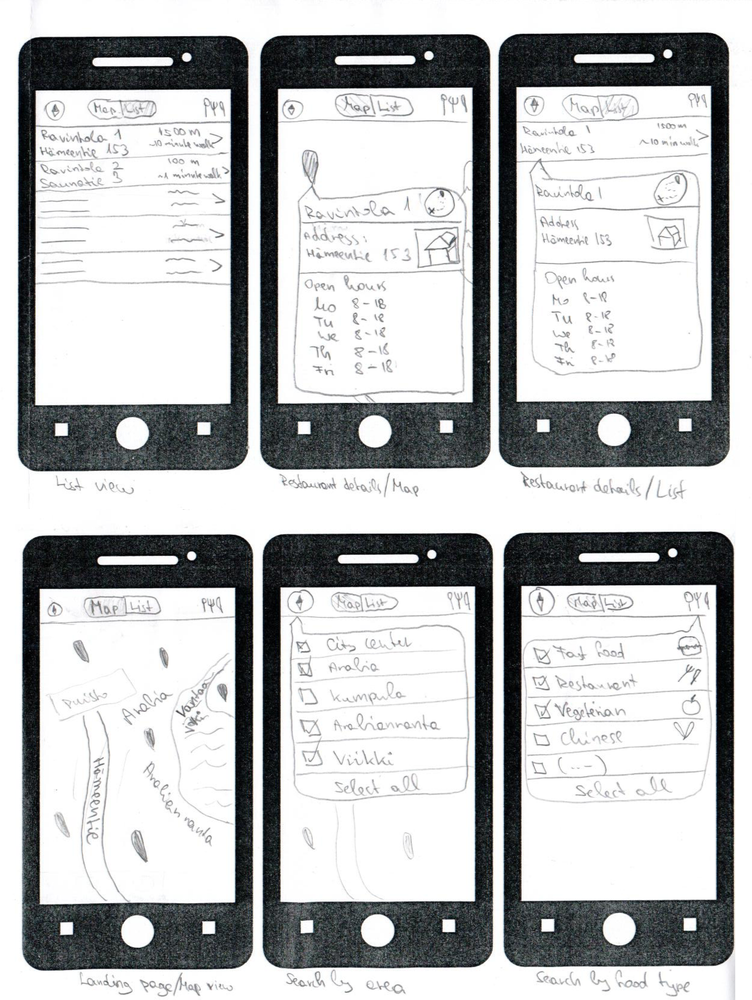
\includegraphics[width=0.8\textwidth]{images/sketch-1.png}
			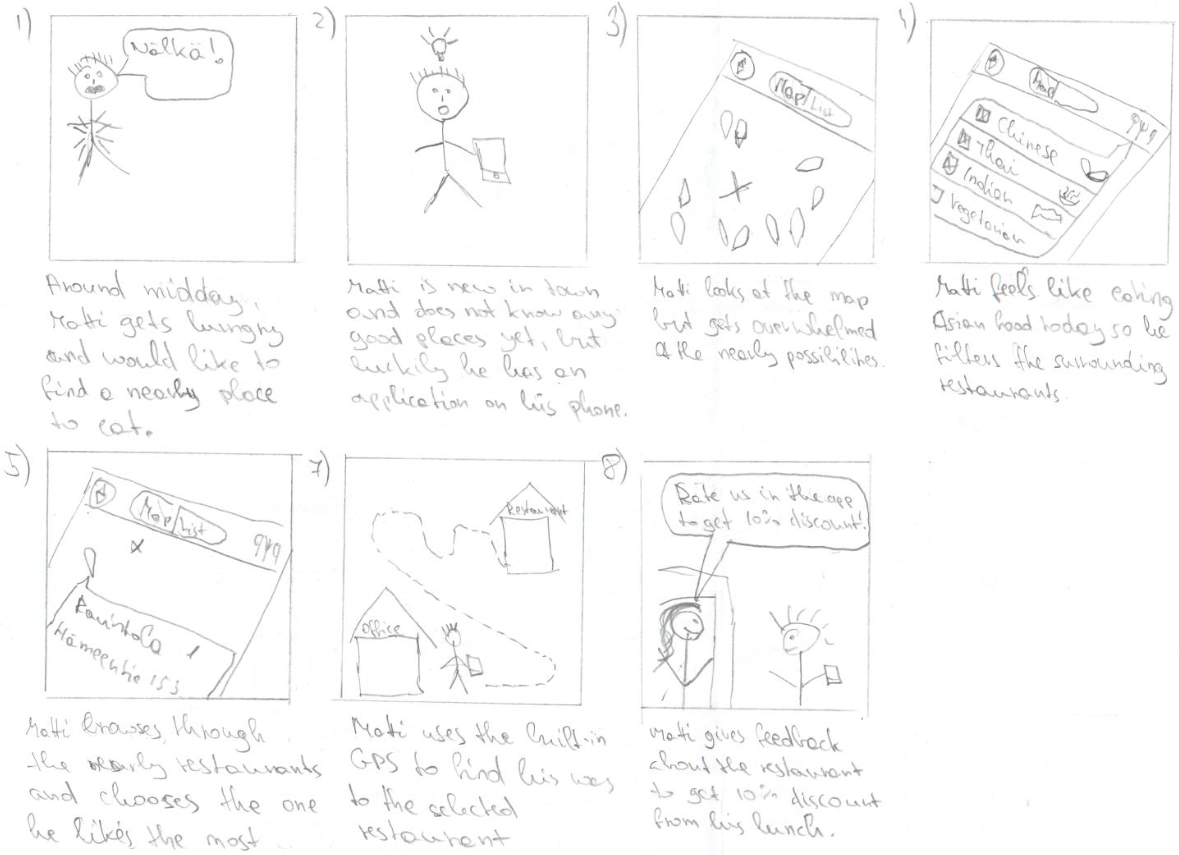
\includegraphics[width=0.8\textwidth]{images/WP_20161125_19_59_47_Pro.jpg}
			\caption{Sketch and Storyboard 1 of the restaurant finder mobile application.}
			\label{sketch-1}
		\end{center}
	\end{figure}
	
	After completing the first sketch, the second sketch was drawn (Figure \ref{sketch-2}). There are slight differences in the design compared to the first sketch, which are explained, as follows.
	
	The landing page is designed differently as it has a combined textbox and a dropdown control. Users are expected to start typing the area they are interested to find restaurants in. While typing, the dropdown menu should be displayed giving suggestions already for successful results. Optionally, they can tap on the arrow on the right side and pick areas they like. Selected areas should be indicated with tickmarks as well as "wells"/"tags" in the textbox above. 
	
	Choosing restaurant categories can be done through the checkboxes below the textbox. The concept is similar as on the first design, consistently following the pictograms on the right and checkmarks on the left side. As there can be multiple possible categories, this list should be scrollable. 
	
	Tapping on the magnifier in the top right corner would navigate forward to the Map view with the hits. On the bottom of the screen users can switch between the List and Map view on the bottom of the screen. The results are displayed on the map and the list similarly as in the first sketch. 
	
	An alternative design is shown for the restaurant details is introduced for the second sketch. The restaurant's name is displayed in the navigation bar, followed by multiple images of the restaurant (e.g. front door, cassa, some photos of ready menus etc.). If there are more pictures than what can fit on the screen, vertical scrolling should be available. Tapping on one of the images would open the images in a full-screen view. Below the images, the address and the opening hours are shown, while the button in the top-right corner would start the navigation to the restaurant respectively. 
	
	Compared to the first sketch (Figure \ref{sketch-1}), the second sketch (Figure \ref{sketch-2}) uses more full-page screens rather than popups. For this reason, a "Back" button is placed in the left side of the navigation in every case to allow users escaping from the current screen. On top of that, it does not present the user the map right away, but asks them to set up filters first. 
	
	\begin{figure}[h] 
		\begin{center}
			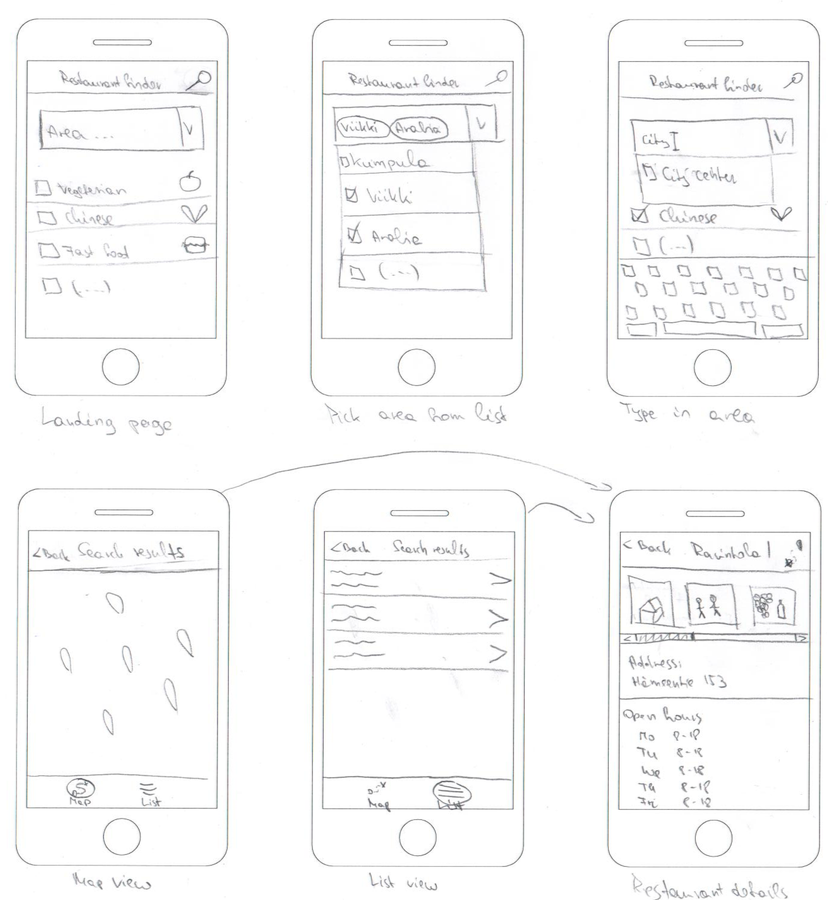
\includegraphics[width=0.8\textwidth]{images/sketch-2.png}
			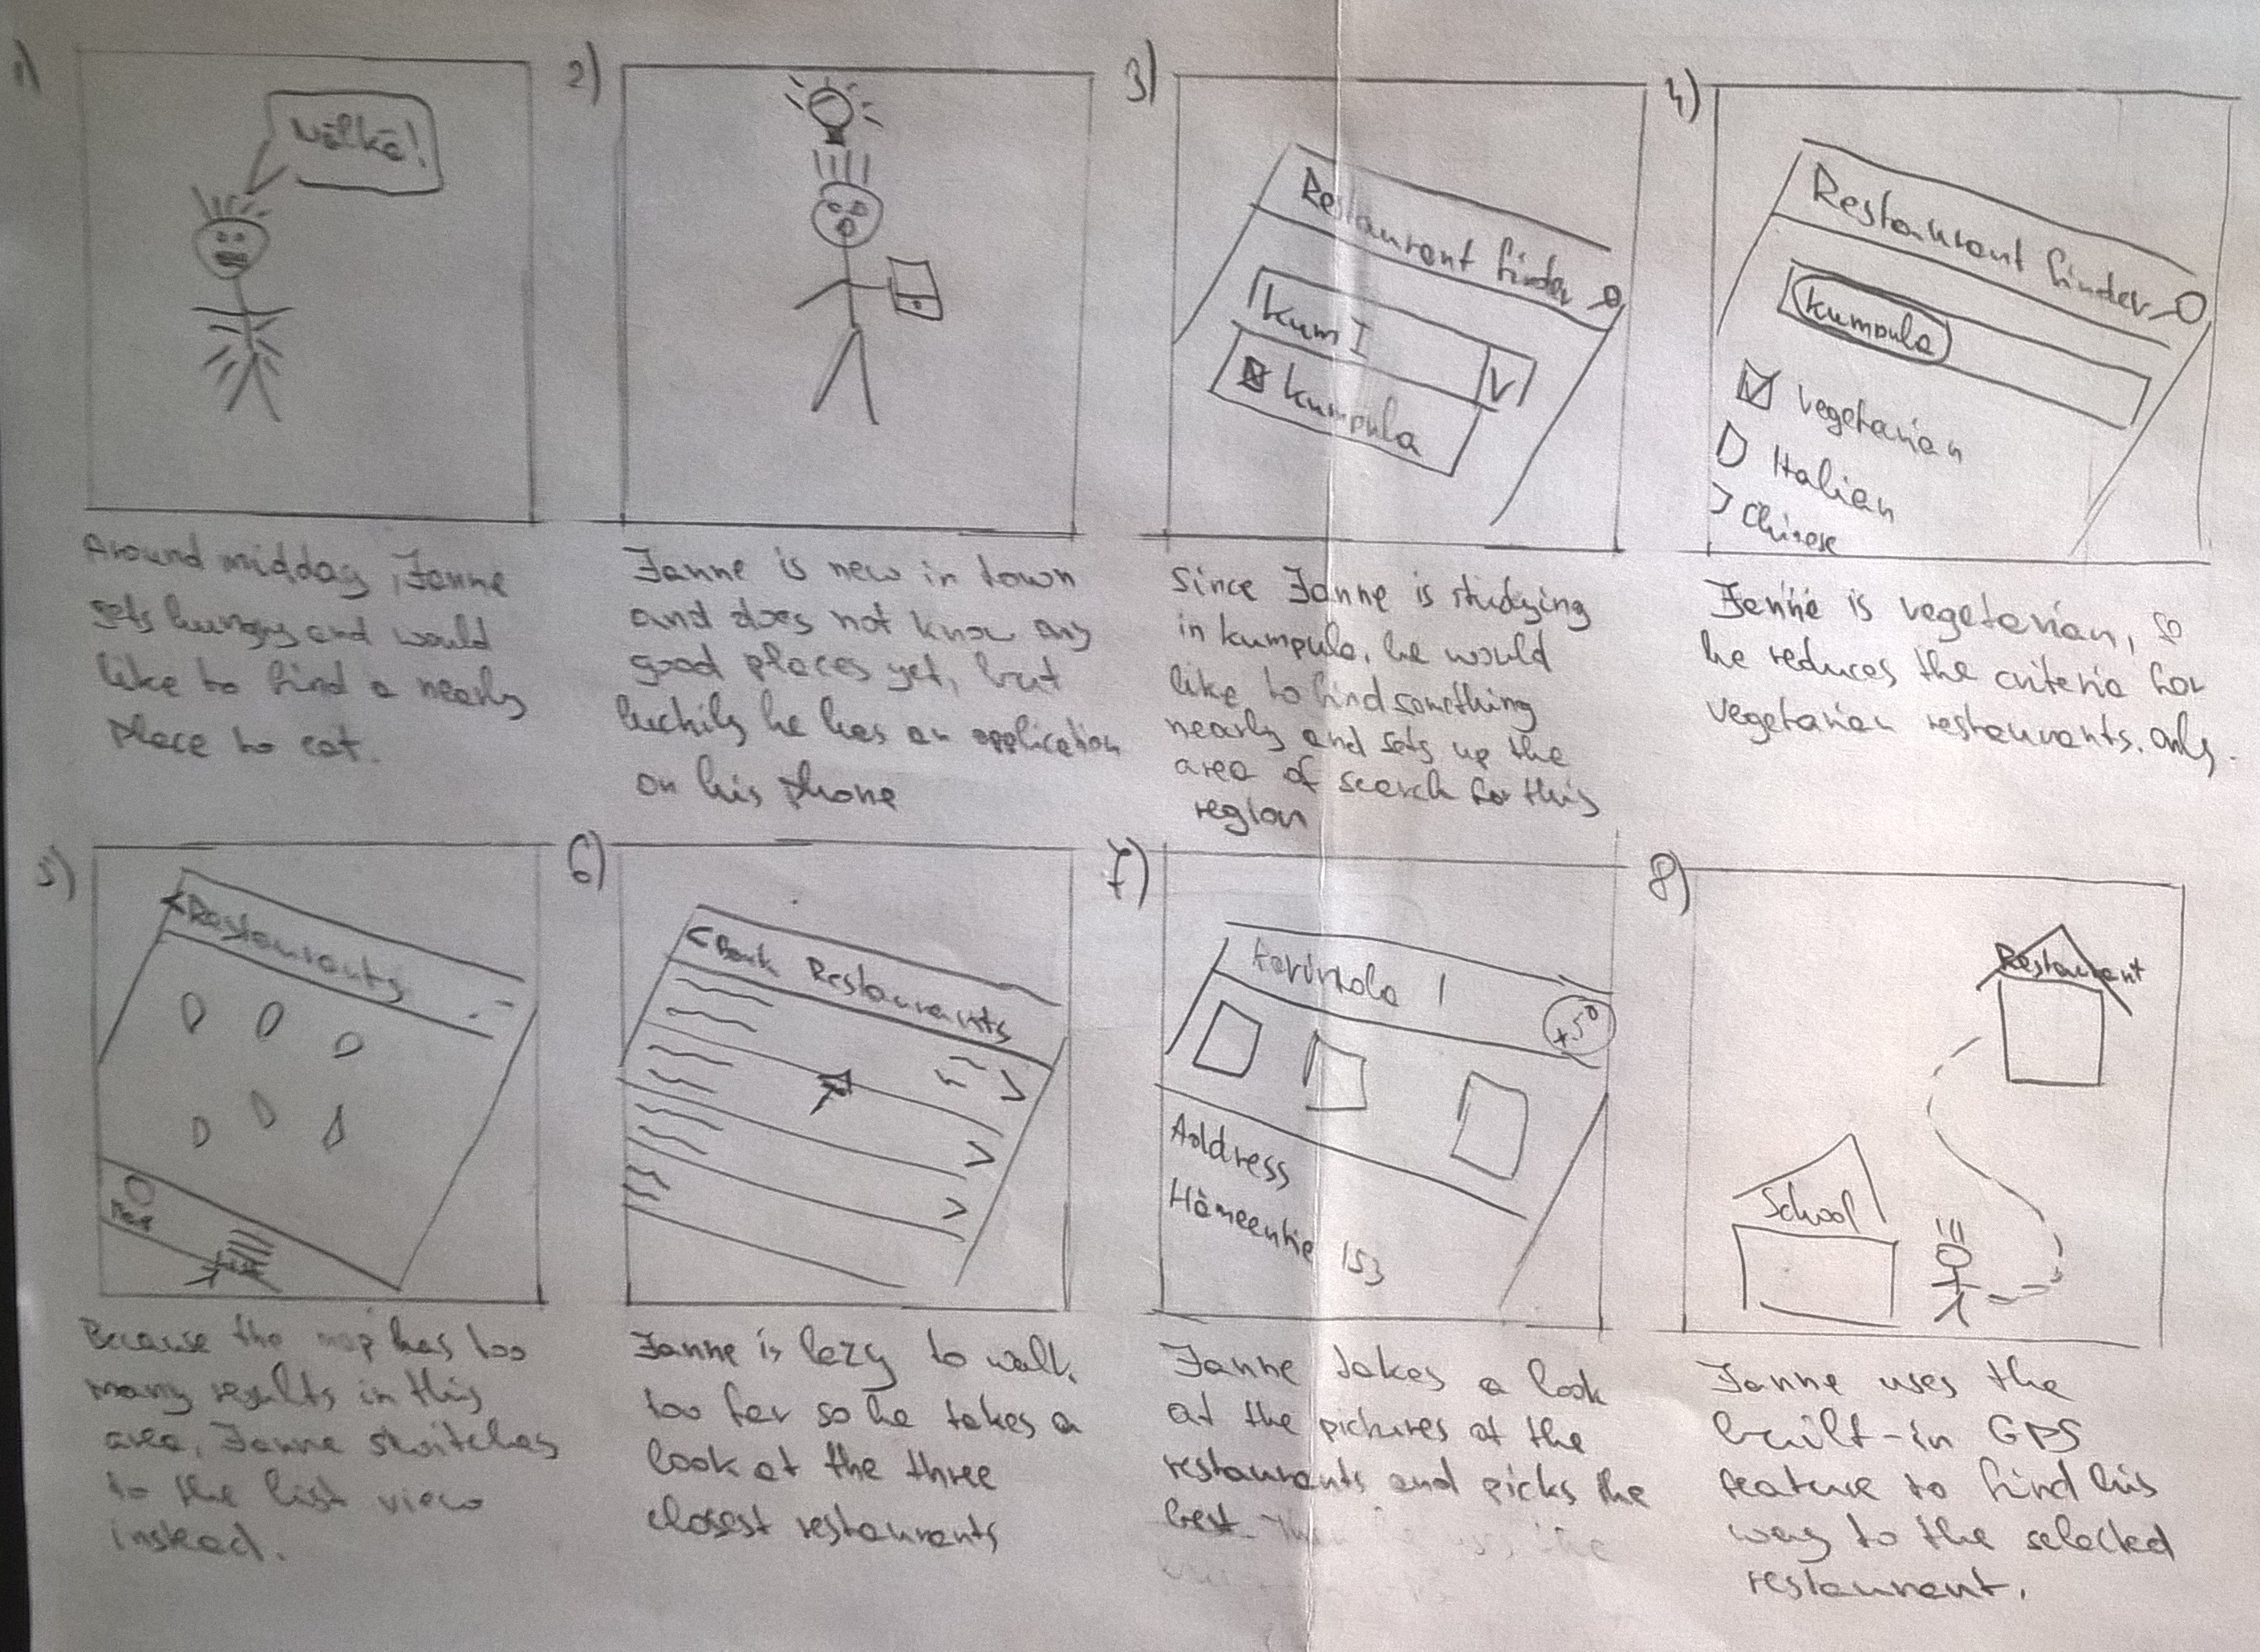
\includegraphics[width=0.8\textwidth]{images/WP_20161125_20_00_06_Pro.jpg}
			\caption{Sketch and Storyboard 2 of the restaurant finder mobile application.}
			\label{sketch-2}
		\end{center}
	\end{figure}
	
	\subsection{Prototype}
	To create the prototype, I decided to merge some of the components of the proposed designs in the sketches. I kept the landing screen and the filtering from sketch 1 (Figure \ref{sketch-1}) and merged it together with the "Restaurant details" screen from sketch 2 (Figure \ref{sketch-2}). 
	
	The reason behind this is the fact that I realized, that the last screen may display more information about the restaurants than I thought at first. For example, the functionality of the application could be extended with ratings, feedback, comments by other users, menus of the restaurant and so on. Accordingly, the amount of information can be a bit more than what is possible to present in a small popup and a full-page design fits for this purpose better. 
	
	The final prototype is shown on Figure \ref{prototype}. I took a copy of both of my sketches and used scissors to cut off the necessary screens. This way we could even perform a usability testing on paper with test users in the future using this material. 
	
	In my opinion this proposal is a good design, because
	
	\begin{itemize}
		\item it is clean, aesthetic, simple, easy to understand,
		\item it is easy to learn and memorable,
		\item it takes advantage of metaphors (i.e. the pictograms next to the food categories),
		\item it does not provide too many possibility for errors,
		\item it models the real world with well-understood abstractions.
	\end{itemize}
		
	\begin{figure}[h] 
		\begin{center}
			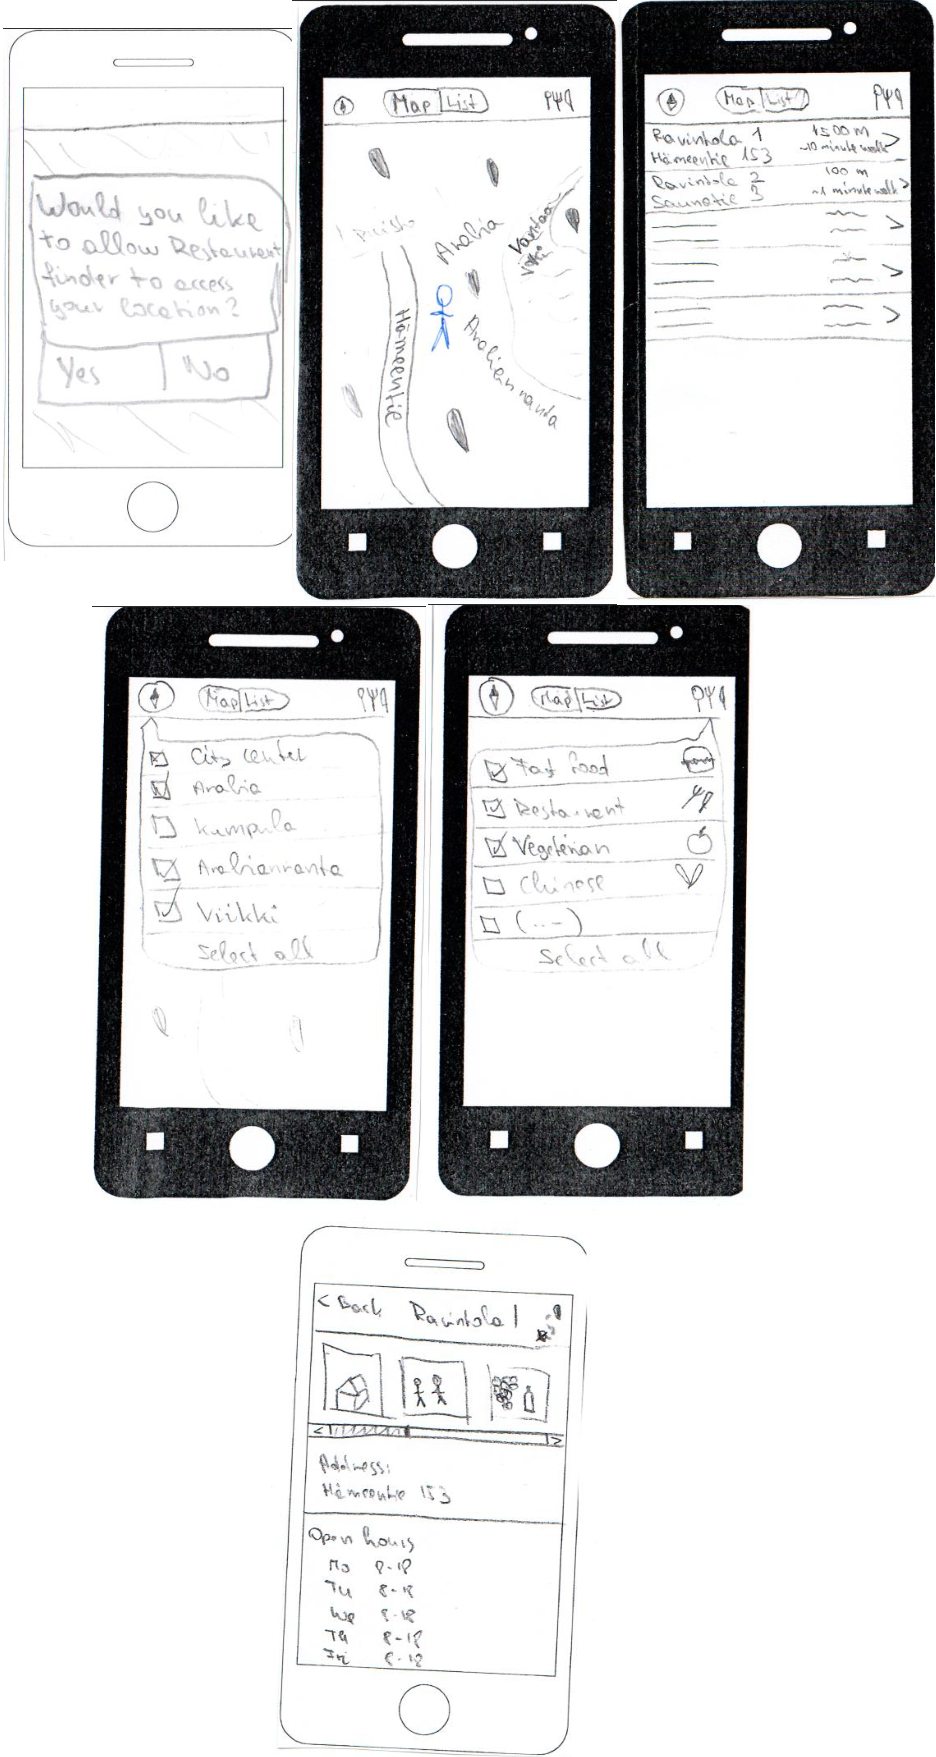
\includegraphics[width=0.8\textwidth]{images/prototype.png}
			\caption{The paper-based prototype of the restaurant finder application.}
			\label{prototype}
		\end{center}
	\end{figure}

\section{Conclusions}
	To conclude, two different sketches for the restaurant finder application were made. The sketches share some similarities, however there are some slight differences between them as well. For both sketches, a storyboard was made which tells a very simple use case of the applicaiton. Finally, a prototype was created by merging the drawings created for the sketches. 
	
	As I proceeded through the points, I realized that some of the approaches may not be the best in the sketches. This way I could design the first prototype more wisely and eliminate the suboptimal design proposals. On top of that, I recognized some new possible features, such as user feedback, discount coupons at the restaurant, addition of menus to the restaurant pages etc. It would be interesting to plan a new sketch and prototype based on the new ideas and lessons learned from the first iteration. 
	
%\pagebreak
%\nocite{*}
%\bibliographystyle{tktl}
%\bibliography{bibliography}

\lastpage

\end{document}